% =====================================================================
% Guía del estudiante -- Geometría 7° -- Trimestre I
% Hilo conductor: Escher, el arte de mover figuras
% Temas (propuesta de curriculo/plan-anual.md, sesiones 002-010):
%   angulos, giros, traslaciones, rotaciones, reflexiones, transformaciones,
%   vistas, objetostransformados
% Plan y ejercicios: guia-periodo-I-transformaciones.plan.md
% Las obras de Escher se describen; no se reproducen (derechos de autor).
% Las clases citan los temas con \refguia{tema:...}. No borrar el .aux de esta guía.
% =====================================================================
% BORRADOR: el plan del trimestre está pendiente de aprobación de la docente (generación rápida 2026-09-14).
\documentclass[11pt]{article}
\makeatletter\def\input@path{{../../../../plantillas/estilo/}}\makeatother
\usepackage{mmcantillo}

% ======================== DATOS DE LA GUÍA ============================
\tipodocumento{Guía del estudiante}
\asignatura{Geometría}
\titulo{Escher: el arte de mover figuras}
\grado{7°}
\periodo{I}
\hiloconductor{Escher: el arte de mover figuras}
% ======================================================================
% DBA: matematicas grado 7 · DBA 5 — Observa objetos tridimensionales desde diferentes puntos de
% vista, los representa según su ubicación y los reconoce cuando se transforman mediante
% rotaciones, traslaciones y reflexiones. (dba/matematicas/grados/grado07.tex)

% Un cubo en perspectiva caballera: \cubo{x}{y}{z}
\newcommand{\cubo}[3]{%
  \filldraw[fill=white] (#1,#2,#3) -- ++(1,0,0) -- ++(0,0,1) -- ++(-1,0,0) -- cycle;
  \filldraw[fill=gray!25] (#1,#2,#3+1) -- ++(1,0,0) -- ++(0,1,0) -- ++(-1,0,0) -- cycle;
  \filldraw[fill=gray!55] (#1+1,#2,#3) -- ++(0,1,0) -- ++(0,0,1) -- ++(0,-1,0) -- cycle;}

\begin{document}

\encabezado

% ---------------------------------------------------------------------
% 1. Frase introductoria
% ---------------------------------------------------------------------
% verificado: https://www.quantamagazine.org/marjorie-rices-secret-pentagons-20170711/ — Wolchover, Quanta, 11 jul. 2017: «I thought, my, that must be wonderful that someone could discover these things which no one had seen before, these beautiful patterns»
\frase{Pensé: qué maravilloso debe ser que alguien pueda descubrir estas cosas que nadie había
visto antes, estos patrones hermosos.}
{Marjorie Rice, en \emph{Quanta Magazine} (2017), trad. propia}

% ---------------------------------------------------------------------
% 2. Introducción
% ---------------------------------------------------------------------
\seccion{Introducción}

Un estampado que se repite en una camiseta, el reflejo de un edificio en un charco, la rueda de
la fortuna que da vueltas, un personaje de videojuego que cambia de dirección: en todos ellos
una figura se \textbf{mueve} sin cambiar de forma ni de tamaño. Este trimestre vamos a estudiar
esos movimientos ---las \textbf{traslaciones}, las \textbf{rotaciones} y las
\textbf{reflexiones}--- primero en el plano y después con objetos de tres dimensiones, vistos
desde distintos lugares.

Nuestro hilo conductor es la obra del artista holandés \textbf{M.~C. Escher}, que pasó buena
parte de su vida llenando hojas con figuras que encajan unas con otras sin dejar huecos, y
dibujando mundos que se ven distintos según desde dónde se los mire. Sus grabados tienen derechos
de autor, así que no los reproducimos aquí: los describimos, y puedes buscarlos por su nombre.

\textbf{Al terminar este trimestre podrás:}
\begin{itemize}
  \item usar el ángulo como medida de un giro, con su sentido;
  \item trasladar, rotar y reflejar figuras en el plano cartesiano, y combinar esos movimientos;
  \item reconocer que las figuras transformadas son congruentes con la original;
  \item dibujar las vistas de un objeto y reconocer un objeto cuando se gira o se refleja.
\end{itemize}

Este trimestre trabaja el siguiente Derecho Básico de Aprendizaje del Ministerio de Educación
Nacional~\cite{mendba}:

\begin{dba}[Grado 7 · DBA 5]
Observa objetos tridimensionales desde diferentes puntos de vista, los representa según su
ubicación y los reconoce cuando se transforman mediante rotaciones, traslaciones y reflexiones.
\end{dba}

% ---------------------------------------------------------------------
% 3. Marco teórico
% ---------------------------------------------------------------------
\seccion{Marco teórico}

\subsubsection*{Un estudiante en la Alhambra}

El 19 de octubre de 1922, Maurits Cornelis Escher, un estudiante holandés de artes gráficas de
24 años, pasó la tarde en la Alhambra, el palacio del siglo XIV en Granada (España), copiando un
mosaico de la pared con una estrella de 16 puntas. Al día siguiente lo terminó con
acuarelas~\cite{museo,aramco}.

\subsubsection*{La segunda visita y la división del plano}

En mayo de 1936 Escher volvió a la Alhambra con su esposa, Jetta. Durante tres días los dos
llenaron cuadernos con notas y dibujos de los mosaicos~\cite{aramco}. A Escher le admiraba que
esos artistas llenaran por completo una pared con figuras iguales que encajan. Como allí solo
hay formas geométricas, él se propuso hacer lo mismo con figuras reconocibles: pájaros, peces,
lagartos~\cite{museo}. Desde entonces practicó durante años lo que llamó la \emph{división regular
del plano}.

Lo que hacía Escher tiene nombre matemático. Cada baldosa de sus dibujos es una copia de otra
que se ha \textbf{trasladado}, \textbf{girado} o \textbf{reflejado}: movimientos que no cambian ni
el tamaño ni la forma. Por eso todas las figuras de un teselado de Escher son
\textbf{congruentes}.

\subsubsection*{Dos matemáticas y los mosaicos}

La matemática estadounidense \textbf{Doris Schattschneider} estudió los cuadernos de Escher y
explicó cómo construyó cada uno de sus dibujos periódicos en el libro \emph{Visions of
Symmetry}~\cite{schattschneider1990}. Ella fue también quien revisó el trabajo de
\textbf{Marjorie Rice}, una señora de San Diego que no había estudiado matemáticas después del
colegio. En 1975, Rice leyó en la revista \emph{Scientific American} un artículo de Martin Gardner
sobre los pentágonos que pueden cubrir un piso sin dejar huecos. Inventó su propia notación y
encontró cuatro tipos nuevos de esos pentágonos; con ellos pintó mosaicos al estilo de Escher.
Hoy se sabe que existen exactamente 15 tipos de pentágonos convexos que cubren el plano: lo
demostró el matemático Michaël Rao en 2017~\cite{quanta,schattschneider2018}.

\subsubsection*{Mundos vistos desde varios lados}

En \emph{Relatividad} (julio de 1953), Escher dibujó un edificio de escaleras en el que lo que es
pared para unos personajes es piso para otros: la misma construcción, vista con tres «arribas»
distintos. En \emph{Reptiles} (marzo de 1943), unos lagartos salen de un dibujo plano de
teselado, caminan en tres dimensiones sobre los objetos de un escritorio y vuelven a entrar al
dibujo~\cite{mcescher}. Esas dos obras nos acompañarán al final del trimestre, cuando pasemos
del plano a los objetos.

% ---------------------------------------------------------------------
% 4. Temas
% ---------------------------------------------------------------------
\tema{Ángulos}\label{tema:angulos}

\begin{hilo}
La estrella de 16 puntas que Escher copió en 1922 está hecha de ángulos: cada punta es un ángulo
agudo y, entre dos puntas, se abre un ángulo entrante. Antes de mover figuras, repasemos cómo se
nombran los ángulos.
\end{hilo}

\begin{definicion}[Ángulo y su clasificación]
Un \textbf{ángulo} está formado por dos rayos con el mismo origen, el \textbf{vértice}. Según su
medida en grados es \textbf{agudo} (menor que $90^\circ$), \textbf{recto} ($90^\circ$),
\textbf{obtuso} (entre $90^\circ$ y $180^\circ$), \textbf{llano} ($180^\circ$),
\textbf{entrante} (entre $180^\circ$ y $360^\circ$) o \textbf{completo} ($360^\circ$).
\end{definicion}

Cuando dos rectas se cortan, los ángulos vecinos (\textbf{adyacentes}) suman $180^\circ$ y los
\textbf{opuestos por el vértice} son iguales.

\begin{center}
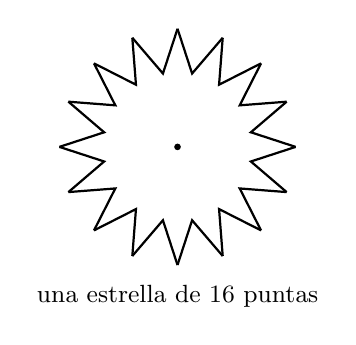
\begin{tikzpicture}
  \foreach \k in {0,...,15} {
    \pgfmathsetmacro{\a}{\k*22.5}
    \pgfmathsetmacro{\b}{\k*22.5+11.25}
    \pgfmathsetmacro{\c}{\k*22.5+22.5}
    \draw[thick] (\a:1.5) -- (\b:0.95) -- (\c:1.5);
  }
  \fill (0,0) circle (1.2pt);
  \node[font=\small] at (0,-1.9) {una estrella de 16 puntas};
\end{tikzpicture}
\end{center}

\begin{aplicacion}[Ángulos en un mosaico]
Los artesanos que diseñan mosaicos de estrellas trabajan con ángulos que dividen la vuelta en
partes iguales. En una estrella de 16 puntas, las puntas están separadas
$360^\circ \div 16 = 22{,}5^\circ$. Con ángulos de $45^\circ$, $90^\circ$ y $22{,}5^\circ$ se arman
muchos de los mosaicos geométricos de la Alhambra.
\end{aplicacion}

\begin{preguntas}
% Ejercicio: angulos-6-002 (del banco de 6°, como repaso)
\pregunta Demuestra que si dos ángulos suplementarios son iguales, entonces cada uno es un
ángulo recto.
\renglones{3}
% Ejercicio: angulos-6-003 (del banco de 6°, como repaso)
\pregunta Demuestra que si dos ángulos complementarios son iguales, entonces cada uno mide
$45^\circ$.
\renglones{3}
\end{preguntas}

\begin{resumen}
\begin{itemize}
  \item Un ángulo son dos rayos con un vértice común; se mide en grados.
  \item Agudo, recto, obtuso, llano, entrante y completo, según su medida.
  \item Los adyacentes suman $180^\circ$; los opuestos por el vértice son iguales.
\end{itemize}
\end{resumen}

% ---------------------------------------------------------------------
\tema{Ángulos y giros}\label{tema:giros}

\begin{hilo}
Si giramos la estrella de la Alhambra alrededor de su centro, en algún momento vuelve a verse
igual. Para decir cuánto hay que girarla, el ángulo deja de ser una abertura quieta y se
convierte en la medida de un movimiento.
\end{hilo}

\begin{definicion}[Giro]
Un \textbf{giro} alrededor de un punto se describe con un \textbf{ángulo} y un \textbf{sentido}:
\textbf{antihorario} (contrario a las manecillas del reloj, el sentido que se usa en matemáticas
como positivo) u \textbf{horario}. Un giro de $360^\circ$ es una vuelta completa y deja todo como
estaba.
\end{definicion}

\begin{ejemplo}[Giros equivalentes]
Girar $270^\circ$ en sentido antihorario deja una figura en la misma posición que girarla
$90^\circ$ en sentido horario, porque $270^\circ + 90^\circ = 360^\circ$. En general, un giro de
$a$ grados en un sentido equivale a uno de $360^\circ - a$ en el sentido contrario.
\end{ejemplo}

\begin{aplicacion}[Relojes y ruedas]
El minutero de un reloj da una vuelta en 60 minutos, así que gira $360^\circ \div 60 = 6^\circ$
cada minuto. Una rueda de la fortuna con 12 cabinas iguales gira $30^\circ$ cada vez que una
cabina ocupa el lugar de la siguiente. Los ingenieros que programan un robot o un brazo mecánico
le dan instrucciones de este tipo: «gira $45^\circ$ en sentido antihorario».
\end{aplicacion}

\begin{preguntas}
% Ejercicio: angulos-7-003 (nuevo: el banco no tenía nada para este tema)
\pregunta Laura dice que girar una figura $270^\circ$ en sentido antihorario la deja en la misma
posición que girarla $90^\circ$ en sentido horario. ¿Tiene razón? Explica con la vuelta completa
y compruébalo girando una escuadra.
\renglones{4}
\end{preguntas}

\begin{resumen}
\begin{itemize}
  \item Un giro se describe con un centro, un ángulo y un sentido (horario o antihorario).
  \item Un giro de $360^\circ$ deja la figura igual.
  \item Girar $a$ en un sentido equivale a girar $360^\circ - a$ en el contrario.
\end{itemize}
\end{resumen}

% ---------------------------------------------------------------------
\tema{Traslaciones}\label{tema:traslaciones}

\begin{hilo}
En los dibujos de Escher, una misma figura aparece una y otra vez, siempre mirando hacia el
mismo lado, como si se hubiera deslizado sobre el papel. Ese deslizamiento es el movimiento más
sencillo de todos.
\end{hilo}

\begin{definicion}[Traslación]
Una \textbf{traslación} mueve todos los puntos de una figura la misma distancia, en la misma
dirección y el mismo sentido. Se describe con un \textbf{vector} $\langle a, b\rangle$: cada punto
$(x, y)$ se lleva a $(x + a,\, y + b)$. La figura trasladada tiene la misma forma, el mismo
tamaño y la misma orientación que la original.
\end{definicion}

\begin{ejemplo}[Trasladar un triángulo]
El triángulo $P(1, 1)$, $Q(3, 1)$, $R(1, 3)$ trasladado con el vector $\langle 4, 1\rangle$ va a
$P'(5, 2)$, $Q'(7, 2)$, $R'(5, 4)$: a cada primera coordenada se le suma 4 y a cada segunda, 1.

\begin{center}
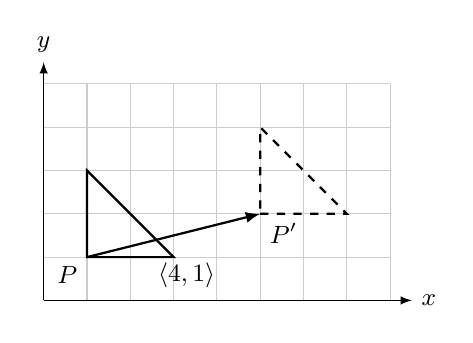
\begin{tikzpicture}[scale=0.55, font=\small, >=latex]
  \draw[gray!40] (0,0) grid (8,5);
  \draw[->] (0,0) -- (8.5,0) node[right] {$x$};
  \draw[->] (0,0) -- (0,5.5) node[above] {$y$};
  \draw[thick] (1,1) -- (3,1) -- (1,3) -- cycle;
  \draw[thick, dashed] (5,2) -- (7,2) -- (5,4) -- cycle;
  \draw[->, thick] (1,1) -- (5,2);
  \node[below left] at (1,1) {$P$}; \node[below right] at (5,2) {$P'$};
  \node[below] at (3.3,1.1) {$\langle 4, 1\rangle$};
\end{tikzpicture}
\end{center}
\end{ejemplo}

\begin{aplicacion}[Estampados y papel de colgadura]
Una máquina de estampar tela imprime el mismo diseño una y otra vez corriendo el rodillo siempre
la misma distancia. El resultado es un patrón hecho con traslaciones: si se desliza la tela un
diseño completo, el patrón coincide consigo mismo.
\end{aplicacion}

\begin{preguntas}
% Ejercicio: transformaciones-7-001 (nuevo: el banco no tenía nada para este tema)
\pregunta Traslada el triángulo de vértices $A(1, 1)$, $B(4, 1)$ y $C(2, 3)$ con el vector
$\langle 3, 2 \rangle$ (3 unidades a la derecha y 2 hacia arriba). Escribe las coordenadas de
$A'$, $B'$ y $C'$ y dibuja las dos figuras.
\espacio{4cm}
\end{preguntas}

\begin{resumen}
\begin{itemize}
  \item Una traslación mueve todos los puntos igual: $(x, y) \to (x + a,\, y + b)$.
  \item Se describe con un vector $\langle a, b\rangle$.
  \item No cambia la forma, el tamaño ni la orientación de la figura.
\end{itemize}
\end{resumen}

% ---------------------------------------------------------------------
\tema{Rotaciones}\label{tema:rotaciones}

\begin{hilo}
La estrella que Escher copió en 1922 tiene 16 puntas iguales. Si se gira alrededor de su centro
la fracción justa de vuelta, cada punta cae donde estaba la siguiente y el mosaico parece no
haberse movido.
\end{hilo}

\begin{definicion}[Rotación]
Una \textbf{rotación} gira todos los puntos de una figura alrededor de un punto fijo, el
\textbf{centro de giro}, un mismo ángulo y en un mismo sentido. El centro es el único punto que
no se mueve. Alrededor del origen, un giro de $90^\circ$ antihorario lleva $(x, y)$ a
$(-y, x)$, y un giro de $180^\circ$ lo lleva a $(-x, -y)$.
\end{definicion}

\begin{ejemplo}[Girar un punto $90^\circ$]
El punto $P(3, 1)$ girado $90^\circ$ en sentido antihorario alrededor del origen va a
$P'(-1, 3)$. Se comprueba con una escuadra: el segmento $OP$ y el segmento $OP'$ miden lo mismo
y forman un ángulo recto.

\begin{center}
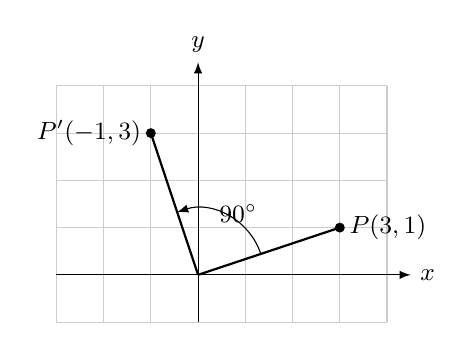
\begin{tikzpicture}[scale=0.6, font=\small, >=latex]
  \draw[gray!40] (-3,-1) grid (4,4);
  \draw[->] (-3,0) -- (4.5,0) node[right] {$x$};
  \draw[->] (0,-1) -- (0,4.5) node[above] {$y$};
  \draw[thick] (0,0) -- (3,1); \draw[thick] (0,0) -- (-1,3);
  \fill (3,1) circle (3pt) node[right] {$P(3,1)$};
  \fill (-1,3) circle (3pt) node[left] {$P'(-1,3)$};
  \draw[->] (18.43:1.4) arc (18.43:108.43:1.4);
  \node at (0.85,1.3) {$90^\circ$};
\end{tikzpicture}
\end{center}
\end{ejemplo}

Una figura tiene \textbf{simetría de rotación} si algún giro menor que $360^\circ$ la deja igual.
El menor de esos giros es $360^\circ$ dividido entre el número de partes iguales que tiene.

\begin{aplicacion}[Rines y logotipos]
El rin de una bicicleta o de un carro con 5 rayos iguales se ve igual cada vez que gira
$360^\circ \div 5 = 72^\circ$. Muchos logotipos se diseñan con simetría de rotación para que se
reconozcan desde cualquier lado.
\end{aplicacion}

\begin{preguntas}
\Needspace{10\baselineskip}
% Ejercicio: transformaciones-7-004 (nuevo: el banco no tenía nada para este tema)
\pregunta Gira el punto $P(3, 1)$ alrededor del origen. Usa papel cuadriculado y una escuadra
para comprobar cada giro.
\begin{opciones*}(3)
  \item $90^\circ$ en sentido antihorario;
  \item $180^\circ$;
  \item $90^\circ$ en sentido horario.
\end{opciones*}
\espacio{3.5cm}
\end{preguntas}

\begin{resumen}
\begin{itemize}
  \item Una rotación se describe con su centro, su ángulo y su sentido.
  \item Alrededor del origen: $90^\circ$ antihorario, $(x, y) \to (-y, x)$; $180^\circ$,
        $(x, y) \to (-x, -y)$.
  \item Una figura con $n$ partes iguales alrededor de un centro se ve igual cada
        $360^\circ \div n$.
\end{itemize}
\end{resumen}

% ---------------------------------------------------------------------
\tema{Reflexiones}\label{tema:reflexiones}

\begin{hilo}
En 1936, Escher y Jetta pasaron tres días dibujando los mosaicos de la Alhambra. En muchos de
ellos una mitad es el reflejo de la otra, como si hubiera un espejo en el medio.
\end{hilo}

\begin{definicion}[Reflexión]
Una \textbf{reflexión} respecto a una recta, el \textbf{eje}, lleva cada punto a otro que está al
otro lado del eje, a la misma distancia, sobre la perpendicular al eje. Respecto al eje $y$,
$(x, y) \to (-x, y)$; respecto al eje $x$, $(x, y) \to (x, -y)$. La figura reflejada es
congruente con la original, pero queda \textbf{invertida}, como en un espejo.
\end{definicion}

Si una figura coincide con su reflejo respecto a una recta, esa recta es un \textbf{eje de
simetría} de la figura. Un triángulo equilátero tiene 3 ejes de simetría; un cuadrado, 4; un
rectángulo que no es cuadrado, 2.

\begin{center}
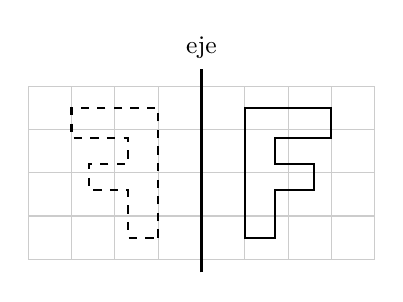
\begin{tikzpicture}[scale=0.55, font=\small]
  \draw[gray!40] (-4,0) grid (4,4);
  \draw[thick] (0,-0.3) -- (0,4.4) node[above] {eje};
  \draw[thick] (1,0.5) -- (1,3.5) -- (3,3.5) -- (3,2.8) -- (1.7,2.8) -- (1.7,2.2) -- (2.6,2.2)
    -- (2.6,1.6) -- (1.7,1.6) -- (1.7,0.5) -- cycle;
  \draw[thick, dashed] (-1,0.5) -- (-1,3.5) -- (-3,3.5) -- (-3,2.8) -- (-1.7,2.8) -- (-1.7,2.2)
    -- (-2.6,2.2) -- (-2.6,1.6) -- (-1.7,1.6) -- (-1.7,0.5) -- cycle;
\end{tikzpicture}
\end{center}

\begin{aplicacion}[La palabra AMBULANCIA]
En el frente de muchas ambulancias la palabra AMBULANCIA está escrita al revés. Así, el
conductor que va adelante la lee derecha en su espejo retrovisor: el espejo hace una reflexión y
la vuelve a invertir.
\end{aplicacion}

\begin{preguntas}
\Needspace{10\baselineskip}
% Ejercicio: transformaciones-7-009 (nuevo: el banco no tenía nada para este tema)
\pregunta Valentina afirma: «reflejar una figura respecto al eje $y$ es lo mismo que girarla
$180^\circ$ alrededor del origen». Encuentra el error con el punto $(2, 3)$ y explica qué
diferencia hay entre las dos figuras que se obtienen con una letra F.
\renglones{4}
\end{preguntas}

\begin{resumen}
\begin{itemize}
  \item Una reflexión se describe con su eje; cada punto va al otro lado, a la misma distancia.
  \item Respecto al eje $y$ cambia de signo la primera coordenada; respecto al eje $x$, la segunda.
  \item La figura reflejada es congruente pero invertida: una reflexión no es un giro.
\end{itemize}
\end{resumen}

% ---------------------------------------------------------------------
\tema{Transformaciones}\label{tema:transformaciones}

\begin{hilo}
Para llenar un plano entero con lagartos o pájaros, Escher combinaba los tres movimientos: una
figura se gira, luego se traslada, luego se refleja\ldots\ y siempre encaja con sus vecinas.
\end{hilo}

\begin{definicion}[Transformaciones rígidas y congruencia]
Traslaciones, rotaciones y reflexiones son \textbf{transformaciones rígidas}: conservan las
longitudes y los ángulos. Aplicar una después de otra se llama \textbf{componer}. Dos figuras son
\textbf{congruentes} si una se puede llevar exactamente sobre la otra con una o varias
transformaciones rígidas.
\end{definicion}

\begin{ejemplo}[Dos traslaciones seguidas]
Trasladar con $\langle 2, 1\rangle$ y después con $\langle -5, 3\rangle$ es lo mismo que trasladar
una sola vez con $\langle 2 + (-5),\, 1 + 3\rangle = \langle -3, 4\rangle$: los vectores se suman.
\end{ejemplo}

Un \textbf{teselado} es un cubrimiento del plano con figuras que no se superponen ni dejan huecos.
Los teselados de Escher empiezan con un polígono que cubre el plano ---un cuadrado, un
paralelogramo, un hexágono--- y lo deforman: lo que se quita de un lado se agrega trasladado,
girado o reflejado en otro lado, así que la baldosa sigue encajando con sus vecinas.

\begin{aplicacion}[Baldosas y pisos]
Las baldosas de un piso cubren el plano con copias congruentes de una misma pieza. Los pentágonos
de Marjorie Rice sirven para pisos: cada uno encaja con sus vecinos después de girarlo o
reflejarlo, y Rice los usó para pintar mosaicos al estilo de Escher~\cite{quanta}.
\end{aplicacion}

\begin{preguntas}
\Needspace{10\baselineskip}
% Ejercicio: transformaciones-7-012 (nuevo: el banco no tenía nada para este tema)
\pregunta Aplica al triángulo $A(0, 0)$, $B(3, 0)$, $C(0, 2)$ un giro de $90^\circ$ antihorario
alrededor del origen y luego una traslación con $\langle 5, 1 \rangle$. Halla la figura final y
compara las longitudes de sus lados con las del triángulo original. ¿Son congruentes? ¿Por qué?
\espacio{4cm}
\end{preguntas}

\begin{resumen}
\begin{itemize}
  \item Traslaciones, rotaciones y reflexiones conservan longitudes y ángulos.
  \item Componer es aplicar una transformación después de otra; dos traslaciones dan una traslación.
  \item Dos reflexiones en ejes perpendiculares equivalen a un giro de $180^\circ$.
  \item Las figuras que se obtienen así son congruentes; un teselado se arma con ellas.
\end{itemize}
\end{resumen}

% ---------------------------------------------------------------------
\tema{Vistas de un objeto}\label{tema:vistas}

\begin{hilo}
En \emph{Relatividad}, Escher dibujó escaleras que unos personajes suben mientras otros las
recorren de lado, porque para cada uno el «arriba» está en otra dirección. Un mismo objeto se ve
distinto según desde dónde se mire.
\end{hilo}

\begin{definicion}[Vistas]
La \textbf{vista frontal} de un objeto es lo que se ve mirándolo de frente; la \textbf{superior},
mirándolo desde arriba; la \textbf{inferior}, desde abajo; y las \textbf{laterales}, desde los
lados. Cada vista es una figura plana.
\end{definicion}

Por ejemplo, una lata de gaseosa (un cilindro) se ve de frente como un rectángulo, y desde arriba
y desde abajo como un círculo. Toma un envase de tu casa, dibuja sus tres vistas y compáralas con
fotos tomadas desde esos tres lugares.

\textbf{Construcciones con cubos.} Una construcción de cubos se describe con su \textbf{plano de
alturas}: la vista superior en una cuadrícula, con el número de cubos apilados en cada casilla.
La vista frontal muestra, en cada columna, la pila más alta.

\Needspace{12\baselineskip}
\begin{ejemplo}[Del plano de alturas a las vistas]
\begin{center}
\begin{minipage}{0.3\linewidth}\centering
\renewcommand{\arraystretch}{1.3}
\begin{tabular}{|c|c|c|}\hline 3 & 1 & 2\\\hline 2 & 1 & 1\\\hline\end{tabular}\\[2pt]
{\footnotesize plano de alturas\\(abajo: la fila de adelante)}
\end{minipage}\hfill
\begin{minipage}{0.36\linewidth}\centering
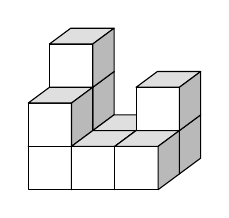
\begin{tikzpicture}[x={(0.55cm,0cm)}, y={(0.27cm,0.2cm)}, z={(0cm,0.55cm)}, line join=round]
  \cubo{0}{1}{0}\cubo{0}{1}{1}\cubo{0}{1}{2}\cubo{1}{1}{0}\cubo{2}{1}{0}\cubo{2}{1}{1}
  \cubo{0}{0}{0}\cubo{0}{0}{1}\cubo{1}{0}{0}\cubo{2}{0}{0}
\end{tikzpicture}\\
{\footnotesize la construcción (10 cubos)}
\end{minipage}\hfill
\begin{minipage}{0.3\linewidth}\centering
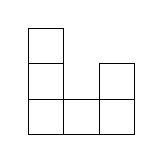
\begin{tikzpicture}[scale=0.45]
  \draw (0,0) grid (1,3); \draw (1,0) grid (2,1); \draw (2,0) grid (3,2);
\end{tikzpicture}\\
{\footnotesize vista frontal: 3, 1, 2}
\end{minipage}
\end{center}
\end{ejemplo}

\begin{aplicacion}[Los planos de una casa]
Los arquitectos no dibujan una casa «en perspectiva» para construirla: entregan su planta (la
vista superior) y sus fachadas (las vistas frontal y laterales), con las medidas. Con esas
vistas, el maestro de obra sabe dónde va cada muro y qué altura tiene.
\end{aplicacion}

\begin{preguntas}
\Needspace{9\baselineskip}
% Ejercicio: vistas-7-001 (nuevo: el banco no tenía nada para este tema)
\pregunta Este plano de alturas muestra una construcción vista desde arriba; cada número dice
cuántos cubos hay apilados en esa casilla (la fila de abajo es la de adelante):
\begin{center}
\renewcommand{\arraystretch}{1.3}
\begin{tabular}{|c|c|c|}\hline 3 & 1 & 2\\\hline 2 & 1 & 1\\\hline\end{tabular}
\end{center}
\begin{opciones*}(1)
  \item ¿Cuántos cubos tiene?
  \item Dibuja su vista frontal y su vista lateral derecha en papel cuadriculado, indicando la
        altura de cada columna.
\end{opciones*}
\espacio{3.5cm}
\end{preguntas}

\begin{resumen}
\begin{itemize}
  \item Las vistas frontal, superior, inferior y laterales son figuras planas del mismo objeto.
  \item Un plano de alturas describe una construcción con cubos.
  \item La vista frontal muestra la pila más alta de cada columna; a veces hay cubos escondidos.
\end{itemize}
\end{resumen}

% ---------------------------------------------------------------------
\tema{Objetos transformados}\label{tema:objetostransformados}

\begin{hilo}
En \emph{Reptiles}, los lagartos de un teselado plano salen del papel, caminan sobre un libro y
otros objetos del escritorio y vuelven a entrar al dibujo. Pasan del plano al espacio sin dejar
de ser los mismos: las transformaciones también sirven para objetos de tres dimensiones.
\end{hilo}

Un objeto de tres dimensiones también se puede \textbf{trasladar} (moverlo sobre la mesa sin
girarlo), \textbf{rotar} (girarlo sobre la mesa alrededor de un eje vertical) o
\textbf{reflejar} (verlo en un espejo). En una construcción de cubos:
\begin{itemize}
  \item al girarla $90^\circ$ sobre la mesa, su plano de alturas gira $90^\circ$ y sus vistas
        cambian, pero el número de cubos no;
  \item al verla en un espejo vertical, el orden de las columnas se invierte, como en una
        reflexión del plano.
\end{itemize}

\begin{ejemplo}[Una torre en el espejo]
Una fila de tres pilas de alturas 1, 2 y 3 (de izquierda a derecha), vista en un espejo colocado
a su derecha, se ve con alturas 3, 2 y 1: la pila más alta, que estaba más cerca del espejo,
aparece en la imagen también más cerca del espejo, es decir, a la izquierda de la imagen.
\end{ejemplo}

\begin{aplicacion}[Modelado 3D y videojuegos]
Los programas de modelado en 3D y los videojuegos guardan un objeto una sola vez y lo muestran
trasladado, girado o reflejado según haga falta: un personaje que corre hacia la izquierda suele
ser el mismo modelo que corre hacia la derecha, reflejado.
\end{aplicacion}

\begin{preguntas}
\Needspace{8\baselineskip}
% Ejercicio: vistas-7-004 (nuevo: el banco no tenía nada para este tema)
\pregunta La construcción del plano de alturas
\begin{center}
\renewcommand{\arraystretch}{1.3}
\begin{tabular}{|c|c|c|}\hline 3 & 1 & 2\\\hline 2 & 1 & 1\\\hline\end{tabular}
\end{center}
se gira $90^\circ$ en sentido horario sobre la mesa (vista desde arriba). Escribe el nuevo plano
de alturas y la nueva vista frontal. ¿Cambió el número de cubos?
\espacio{3.5cm}
\end{preguntas}

\begin{resumen}
\begin{itemize}
  \item Los objetos de tres dimensiones también se trasladan, se giran y se reflejan.
  \item Girar una construcción cambia sus vistas, pero no el número de cubos.
  \item En un espejo, el orden de izquierda a derecha se invierte.
\end{itemize}
\end{resumen}

% ---------------------------------------------------------------------
% 5. Cierre del hilo conductor
% ---------------------------------------------------------------------
\seccion{Cierre: mover sin deformar}

Escher nunca estudió matemáticas en la universidad, pero los matemáticos se reconocieron en su
obra: lo que él llamaba «dividir el plano» es trasladar, girar y reflejar figuras congruentes.
Schattschneider lo explicó con cuidado, y Marjorie Rice, que tampoco era matemática de
profesión, descubrió pentágonos que nadie había visto. Este trimestre recorrimos el mismo camino:
del ángulo al giro, del giro a las tres transformaciones, y del plano a los objetos que se ven
distintos según desde dónde se miren.

En el próximo trimestre ya no moveremos las figuras: cambiaremos su tamaño. Veremos escalas,
planos, mapas y maquetas.

% ---------------------------------------------------------------------
% 6. Evaluación
% ---------------------------------------------------------------------
\matrizevaluacion
  {Describe una traslación con su vector, una rotación con su centro, ángulo y sentido, y una reflexión con su eje; reconoce las vistas de un objeto.}
  {Aplica transformaciones en el plano cartesiano y a construcciones con cubos, y dibuja las vistas de un objeto.}
  {Comprueba sus transformaciones midiendo lados y ángulos antes de dar un resultado por bueno.}
  {Valora el trabajo de artistas y aficionados, como Escher y Rice, en la construcción de la matemática.}

\autoevaluacion

\seguimientodocente

% ---------------------------------------------------------------------
% 7. Referencias
% ---------------------------------------------------------------------
\begin{referencias}
% verificado: https://www.aramcoworld.com/articles/2023/escher-alhambra-infinity — 19 oct. 1922, estrella de 16 puntas copiada y terminada con acuarelas; mayo de 1936, tres días, con Jetta
\bibitem{aramco} AramcoWorld (2023). \emph{Artwork by M.~C. Escher blending math and
  illusion}. Consultado el 15 de septiembre de 2026.
% verificado: https://mcescher.com/gallery/back-in-holland/ — Reptiles, marzo de 1943, litografía; Relativity, julio de 1953
\bibitem{mcescher} The M.~C. Escher Company. \emph{Gallery: Back in Holland (1941--1954)}.
  Consultado el 15 de septiembre de 2026.
% verificado: https://gblumen.mineducacion.gov.co/cgi-bin/koha/opac-detail.pl?biblionumber=4785 — MEN 2016
\bibitem{mendba} Ministerio de Educación Nacional (2016). \emph{Derechos Básicos de
  Aprendizaje V.2: Matemáticas}. Bogotá: MEN.
% verificado: https://escherinhetpaleis.nl/escher-today/wall-mosaic-in-the-alhambra/?lang=en — visita del 19–20 de oct. de 1922; regreso en 1936; la división regular del plano desde 1936
\bibitem{museo} Escher in Het Paleis (museo). \emph{Wall mosaic in the Alhambra}. La Haya.
  Consultado el 15 de septiembre de 2026.
% verificado: https://www.quantamagazine.org/marjorie-rices-secret-pentagons-20170711/ — Wolchover, 11 jul. 2017: frase de Rice; cuatro tipos nuevos; 15 tipos; Rao 2017
\bibitem{quanta} Wolchover, N. (2017, 11 de julio). Marjorie Rice's secret pentagons.
  \emph{Quanta Magazine}.
% verificado: https://openlibrary.org/books/OL1851833M/Visions_of_symmetry — W. H. Freeman, 1990, ISBN 0-7167-2126-0
\bibitem{schattschneider1990} Schattschneider, D. (1990). \emph{Visions of Symmetry: Notebooks,
  Periodic Drawings, and Related Work of M.~C. Escher}. Nueva York: W.~H. Freeman.
% verificado: https://archive.bridgesmathart.org/2018/bridges2018-1.pdf — Rice: sin formación matemática después del colegio; columna de Gardner de julio de 1975; cuatro tipos nuevos
\bibitem{schattschneider2018} Schattschneider, D. (2018). Marjorie Rice and her pentagonal
  tilings. En \emph{Proceedings of Bridges 2018: Mathematics, Art, Music, Architecture,
  Education, Culture} (pp.~1--8).
\end{referencias}

\end{document}
